\documentclass [a4paper,normaltoc,normalfigtabnum, header, espacoumemeio, capchap, capsec, cappre, 12pt,notimes]{abntpoli}

\usepackage[usenames,dvipsnames]{color}
\usepackage{graphicx}
\usepackage{pstricks}
\usepackage{acronym}
\usepackage[brazil]{babel}
\usepackage[T1]{fontenc}
\usepackage{amsmath}
\usepackage{amssymb}
\usepackage{listings}
\usepackage{tocbibind}
\usepackage[labelsep=endash, font=footnotesize]{caption}
\usepackage[num, abnt-emphasize=bf]{abntcitepoli}
\usepackage[final]{listofsymbols}
\usepackage{url}
\usepackage{textcomp}
\usepackage{imakeidx}
\usepackage{subfig}
\usepackage[section]{placeins}
\usepackage{etoolbox}
\usepackage{dsfont} % fontes matem�ticas duplas como N, Z, R, para designar conjuntos
\usepackage[subfigure]{tocloft}
\usepackage[final]{pdfpages}

%\usepackage{cite}


\renewcommand{\familydefault}{\sfdefault}

\makeindex[title=�ndice]


% 

%\renewcommand{\cftfigfont}{Figura }
%\renewcommand{\cfttabfont}{Tabela }
\setcounter{lofdepth}{1}
\setcounter{tocdepth}{3}
\setcounter{secnumdepth}{3}

\newlength\tablelen
\settowidth\tablelen{\tablename\;}
\addtolength\cfttabnumwidth{\tablelen}
\renewcommand\cfttabpresnum{\tablename\;}
\renewcommand\cfttabaftersnum{\,--\;}

\newlength\figlen
\settowidth\figlen{\figurename\;}
\addtolength\cftfignumwidth{\figlen}
\renewcommand\cftfigpresnum{\figurename\;}
\renewcommand\cftfigaftersnum{\,--\;}


\graphicspath{{./figuras/}}

\allowdisplaybreaks


   
   %\lhead{\thechapter}
   
   

\begin{document}
	\pagenumbering{roman}
	
	
\autor{Nome do Autor}
\titulo{T�tulo da Tese}
\orientador{Nome do Orientador}
\local{S�o Paulo}
\areadeconcentracao{Sistemas Eletr�nicos}
\comentario{Tese apresentada � Escola Polit�cnica da \mbox{Universidade} de S�o Paulo para a obten��o do t�tulo de Doutor em Ci�ncias}
\data{Ano}
\capa
\folhaderosto




	\pretextualchapter{Agradecimentos}

Primeiramente, agrade�o ao Prof. ....

Aos colegas ...

Aos meus pais ....

....

Por fim, � quem me financiou.
	
	%\newpage
	\begin{resumo}
   Esta Tese/Disserta��o � sobre....
   Deve conter no m�ximo 500 palavras.
   
   \noindent
   {\bf Palavras-chave}: Palavra-chave 1. Palavra-chave 2. Palavra-chave 3. Palavra-chave 4. Palavra-chave 5. 
 \end{resumo}

\begin{abstract}

\textbf{Thesis title in English}\\

   This Thesis is about....
   It should have maximally 500 words.
   
   \noindent
   {\bf Keywords}: Keyword 1. Keyword 2. Keyword 3. Keyword 4. Keyword 5.
\end{abstract}


	
%	\renewcommand\listfigurename{Lista de Figuras}
	
	\listadefiguras
	\listadetabelas
%	%%% modifica a maneira de apresentar a lista de siglas
	\def\bflabel#1{{{\textsf{#1}}\hfill}}
	\renewenvironment{AC@deflist}[1]%
	      {\if AC@nolist%
		\else%
		    \raggedright\begin{list}{}%
		    {\settowidth{\labelwidth}{\textsf{#1}+8pt}%
		    \setlength{\leftmargin}{\labelwidth}%
		    \setlength{\itemsep}{0.5pt}%
		    \addtolength{\leftmargin}{\labelsep}%
		    \renewcommand{\makelabel}{\bflabel}}%
		 \fi}%
		{\if AC@nolist%
		  \else%
		    \end{list}%
		\fi}%

\pretextualchapter{Lista de Siglas}

\begin{acronym}[NARMAX]
	\acro{USP}[USP]{Universidade de S�o Paulo}
\end{acronym}




	\renewcommand\symheadingname{Lista de S�mbolos}
\renewcommand\symheading{\pretextualchapter{Lista de S�mbolos}}

\opensymdef
	\newsym[S�mbolo 1]{A}{\alpha}
	\newsym[S�mbolo 2]{X}{x}	
\closesymdef


	\listofsymbols	
	%\lhead{\thechapter}
	
	%%% modifica a maneira de apresentar a lista de siglas
	\def\bflabel#1{{{\textsf{#1}}\hfill}}
	\renewenvironment{AC@deflist}[1]%
	      {\if AC@nolist%
		\else%
		    \raggedright\begin{list}{}%
		    {\settowidth{\labelwidth}{\textsf{#1}+8pt}%
		    \setlength{\leftmargin}{\labelwidth}%
		    \setlength{\itemsep}{0.5pt}%
		    \addtolength{\leftmargin}{\labelsep}%
		    \renewcommand{\makelabel}{\bflabel}}%
		 \fi}%
		{\if AC@nolist%
		  \else%
		    \end{list}%
		\fi}%

\pretextualchapter{Lista de Siglas}

\begin{acronym}[NARMAX]
	\acro{USP}[USP]{Universidade de S�o Paulo}
\end{acronym}




	
	\sumario	
	
	%\pagestyle{fancyplain}
	\chapter{Introdu��o}
\label{cap:intro}

\index{problema}
O problema que esta tese aborda .... ~\cite{Kandel2013,Fuglevand1993, Harris1998}. 

Algo importante a saber ao escrever em portugu�s � que os arquivos .tex devem ser salvos com decodifica��o ISO 8859-15.

... \cite{Heckman2012}. 

\section{Objetivos}
\index{objetivos}
\index{exemplo! sigla}
O objetivo central do trabalho apresentado, realizado na \ac{USP} (este foi um exemplo de uso de sigla),  � ...


\section{Estrutura do texto}

\index{estrutura}
Este texto est� organizado da seguinte maneira ... 




		
 	\chapter{Metodologia}
\label{cap:ident}



\index{exemplo de figura}
Exemplo de figura na Fig.~\ref{fig:exemploFig}.
\begin{figure}[ht!]
	\center
	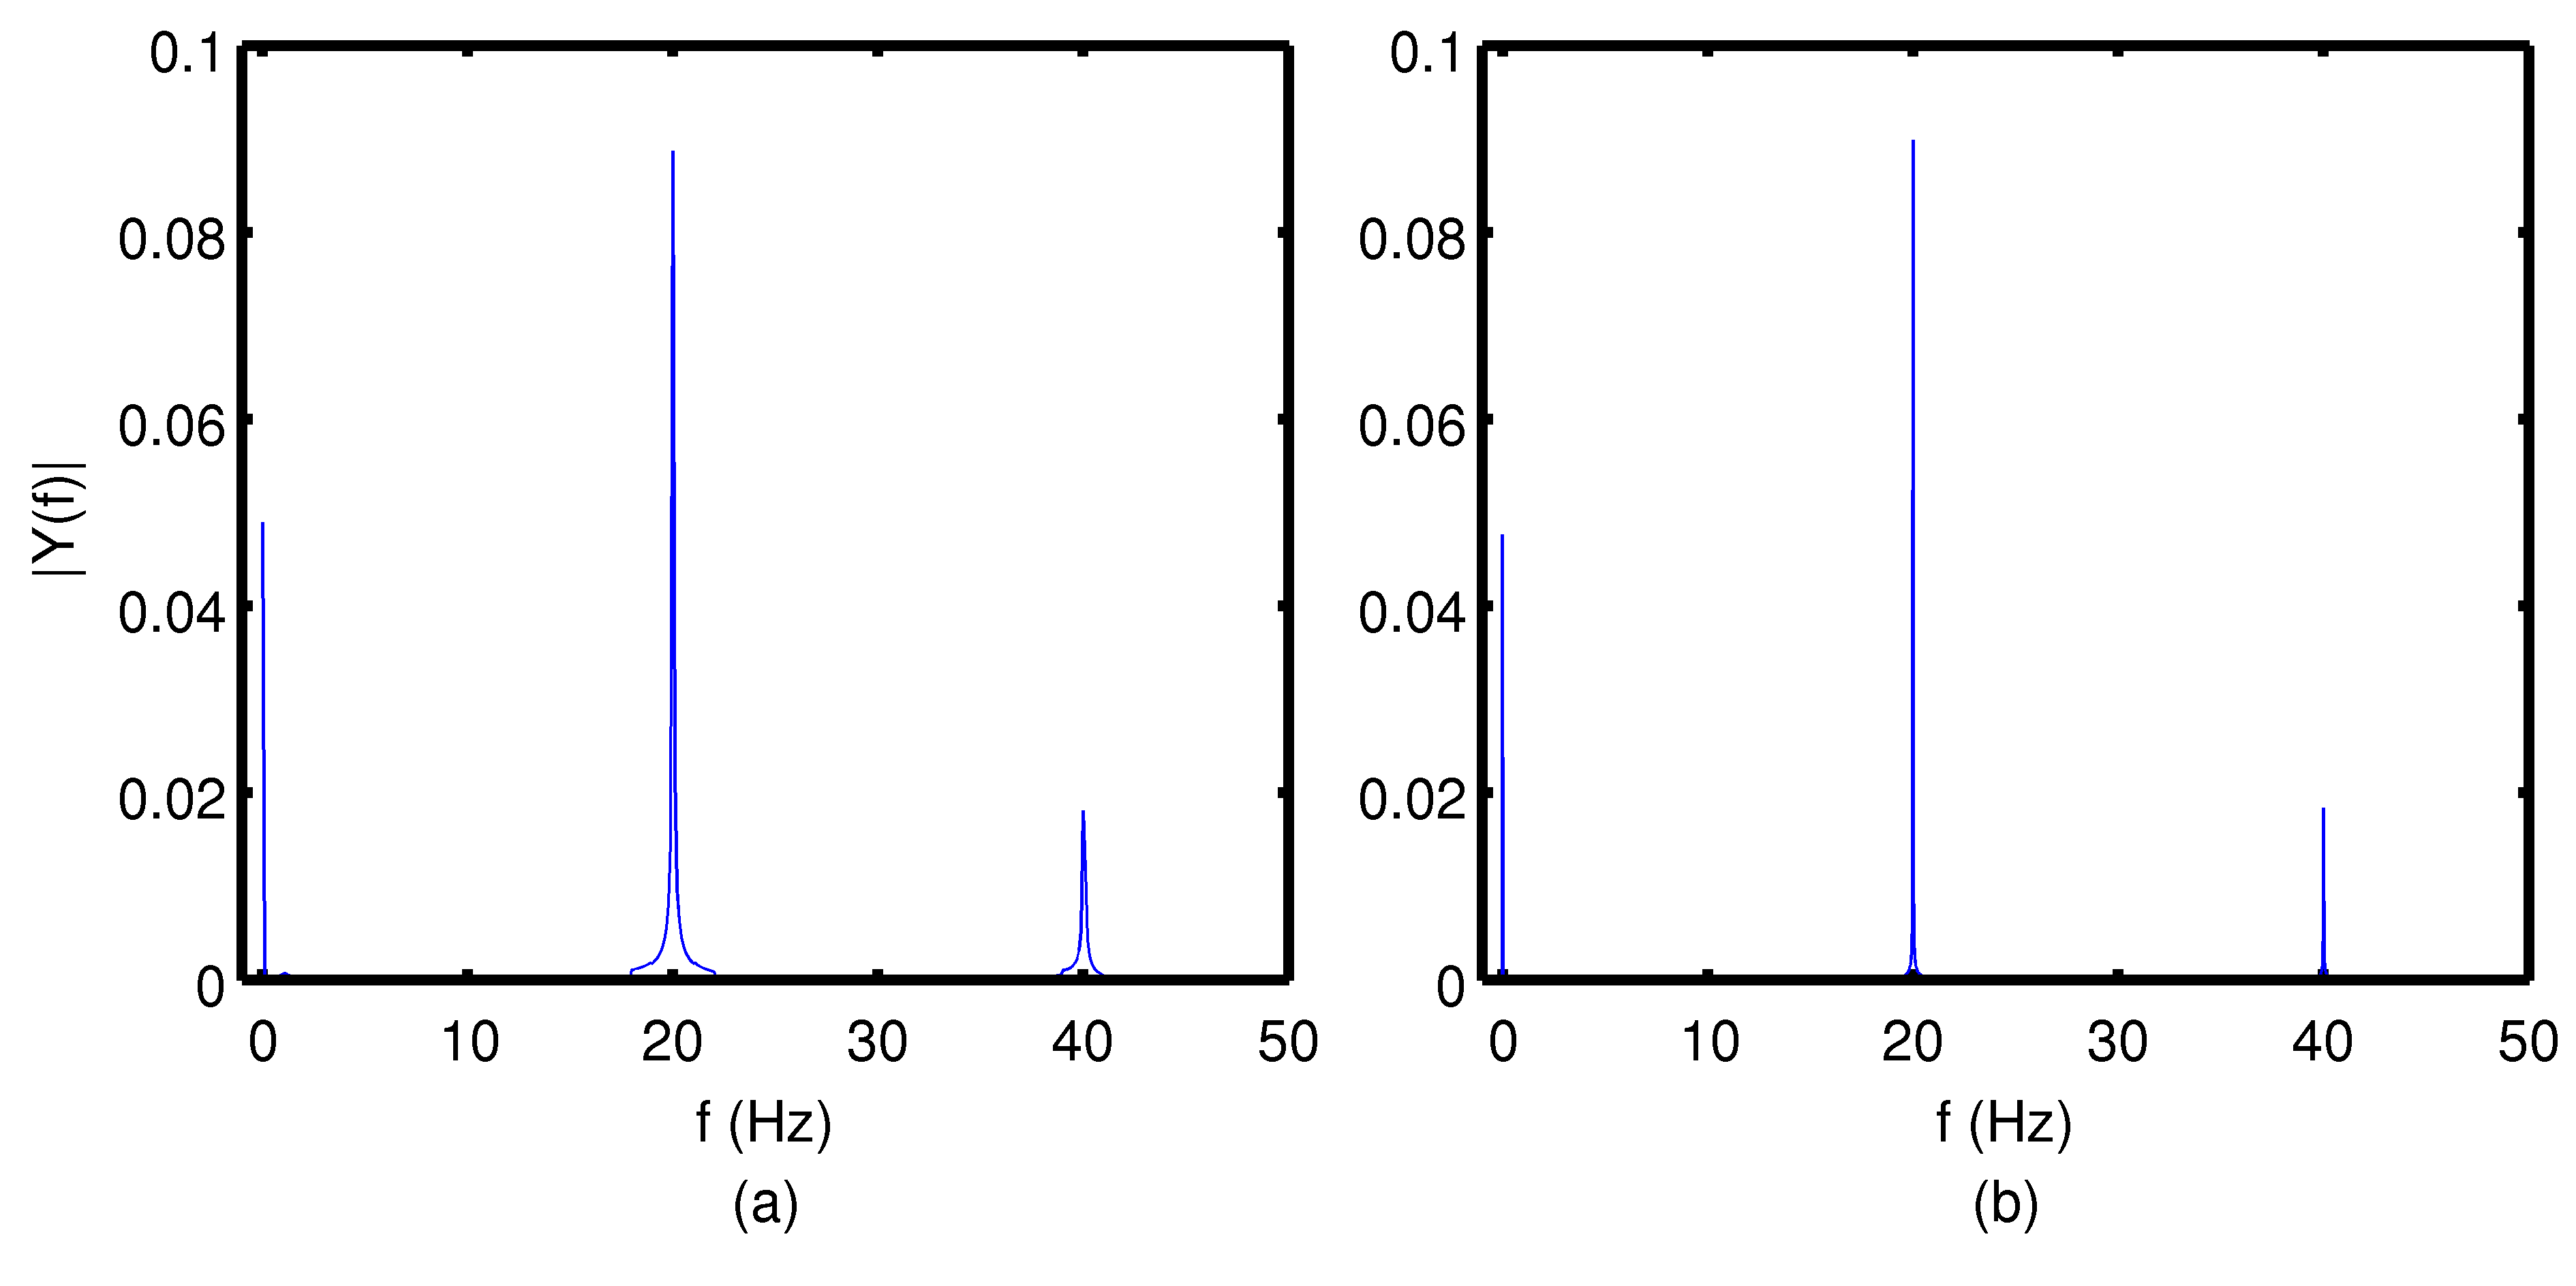
\includegraphics[scale=0.6]{NOFRFExample.png}
	\caption{Exemplo de Figura.}
	\label{fig:exemploFig}
\end{figure}


\index{Exemplo de equa��o}
Exemplo de Equa��o na equa��o~\eqref{eq:exemplo}:
\begin{equation}
  \A = \X + 2
  \label{eq:exemplo}
\end{equation}
 


\section{Mostrando Algoritmo}


\index{Exemplo de algoritmo}
\begin{figure}[!h]
\lstset{keywords=[ 12 ]{func1, indice, naoPertence, para, tamanho, maximo, de, a, se, devolve, soma, e},linewidth=0.95\linewidth,literate={:=}{{$\gets$}}1 {<=}{{$\leqslant$}}1 {>=}{{$\geqslant$}}1 {<>}{{$\neq$}}1 {rho}{{$\rho$}}1   {ws}{{$ws$}}1 {w}{{$w$}}1 {gs_m}{{$gs_m$}}1 {^T}{{$^T$}}1 {^2}{{$^2$}}1 {_s}{{$_s$}}1 {theta}{{$\beta$}}1 {pmatrix}{{\ref{eq:pmatrix}}}1 {^-1}{{$^{-1}$}}1}

\begin{center}
\begin{lstlisting}[frame=single]
func1(param1, param2){
	x := 0
	para (i de 1 a 10){
		x := x + param1 + param2;
	}
	devolve x;	
}
\end{lstlisting}
\end{center}
\vspace{-1.3em}
\caption[Exemplo de Algoritmo]{Exemplo de Algoritmo.}
\label{fig:frols}
\end{figure}

% A matriz $p$, mostrada na Equa��o~\eqref{eq:pmatrix}, quando o modelo segue a representa��o polinomial (Equa��o~\eqref{eq:narmaxpolmodel}), pode ser montada usando o algoritmo na Figura~\ref{fig:pmatrizbuild}. Apesar de parecer simples a montagem desta matriz, achar uma forma geral para o algoritmo n�o foi trivial.  
%

Um exemplo de Tabela � mostrado na Tabela~\ref{tab:exemploTabela}.

\index{Exemplo de Tabela}
\begin{table}[ht!]
\caption{Exemplo de Tabela}
\label{tab:exemploTabela}
\centering
   \begin{tabular}{lrrr}\hline 
	A&B&C&D \\ \hline 
	y(k-1)&2.59e+00&2.44e+00&2.28e+00  \\ 
	y(k-2)&-2.35e+00&-2.12e+00&-1.79e+00  \\ 	
	\hline
    \end{tabular}
\end{table}   






	
	\chapter{Considera��es Finais}
\label{cap:conclusao}

Concluindo, esta Tese/Disserta��o apresentou ....


% 
% 

	
	\ProximoForaDoSumario
	\bibliography{library}
	\setboolean{ABNTNextOutOfTOC}{false}
	
	\apendice
	
	\chapter{Ap�ndice}

\index{ap�ndice}
Este cap�tulo � um Ap�ndice da Tese. Ap�ndices s�o cap�tulos com conte�do criado pelo autor, mas que n�o faz parte do tema central da Tese/Disserta��o.
	
	
	\anexo	
	\chapter{Anexo}


\index{anexo}
Este cap�tulo � um Anexo da Tese. Anexos s�o cap�tulos com conte�do que n�o foi criado pelo autor da Tese/Disserta��o.
	\setboolean{ABNTNextOutOfTOC}{false}
  
  \printindex
	
	
\end{document}

